\section{EXPERIMENTAL EQUIPMENT}
\subsection{Experimental model}
The principle diagram of the experimental model is shown in Figure 1. It is an aerodynamic tube. In which the air is passed from one end of the tube to the other and the temperature is cooled by evaporator of air conditioner, dried by resistor, moistened by spraying vaporized water from the vaporizer.

\subsection{Diagram description}
Air through fan (with flowrate adjustment) 1 passes through aerodynamic tube 2 that is cooled in cooler 4. Then heated and dried in dryer 5, after that, air is moistened by steam nozzle 6 and goes out. In the front and behind positions of each equipment in the aerodynamic tube, there are dry bulbs 7 and wet bulb 8 to measure the temperature and humidity of the air. At the outside aerodynamic tube, there is a speedometer 9 to determine the flowrate of air. Below cooler 4, it is equipped with a volume measuring device to determine the flowrate of the condensed water from cold air.

\begin{figure}[H]
    \centering
    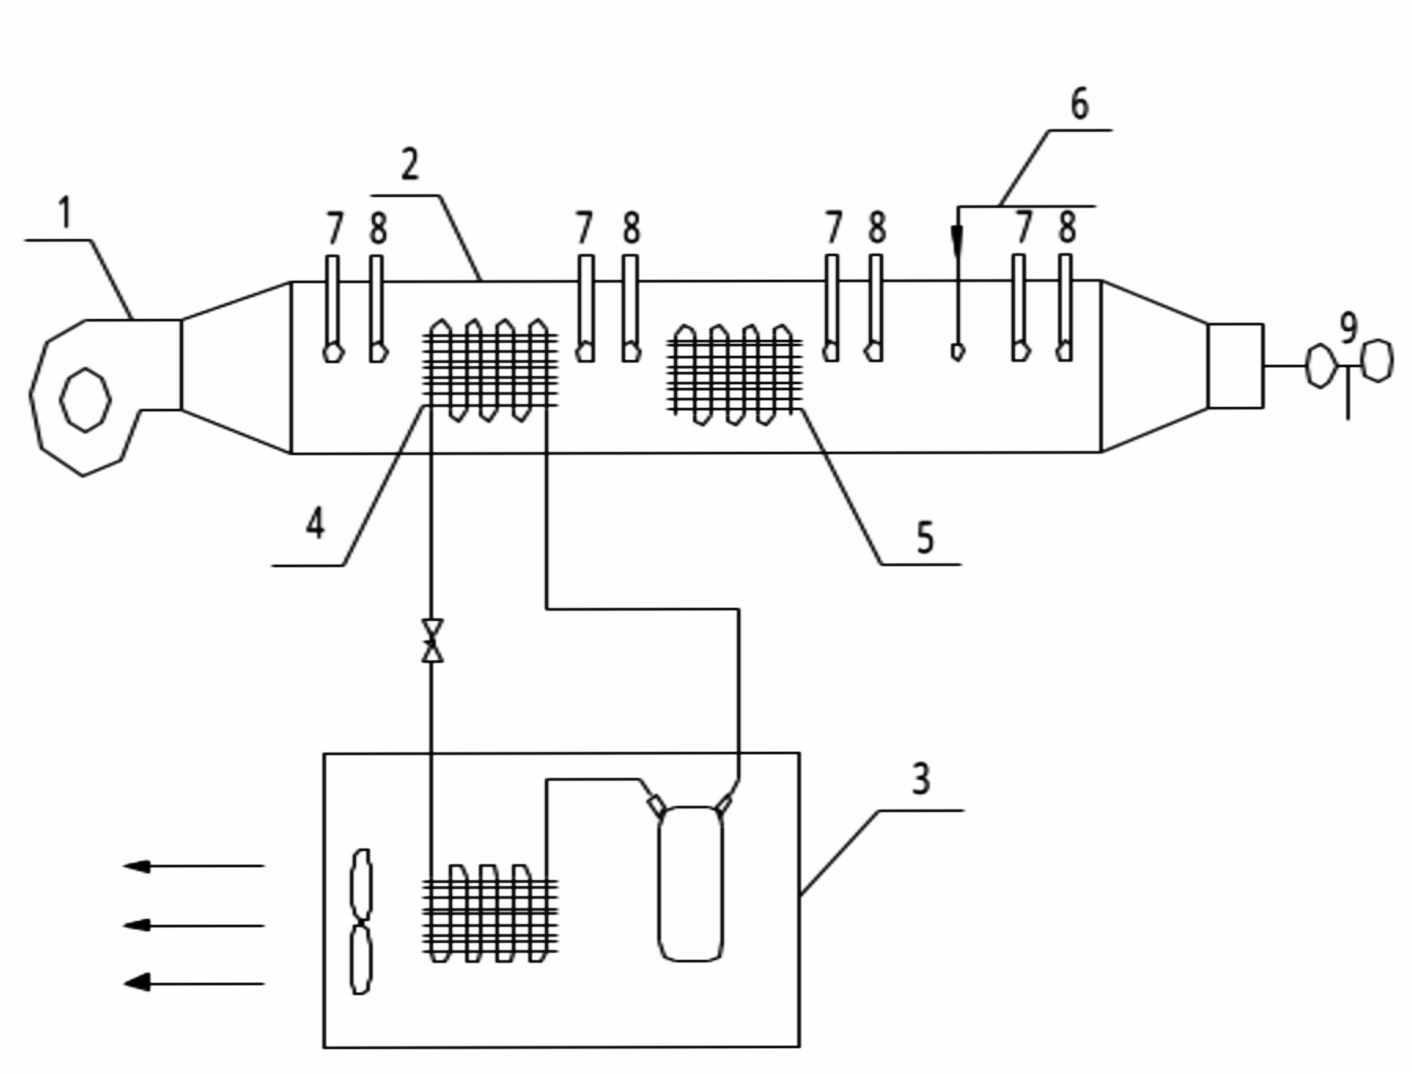
\includegraphics[width=0.8\linewidth]{thermodynamics_appr.png}
    \caption{Experimental diagram of Thermodynamics}
\end{figure}

\begin{itemize}
    \item 1. Fan
    \item 2. Aerodynamic tube
    \item 3. Air conditioner
    \item 4. Cooler
    \item 5. Drying equipment by resistor
    \item 6. Steam nozzle
    \item 7. Dry bulb thermometer
    \item 8. Wet bulb thermometer
    \item 9. Speedometer
\end{itemize}
